\documentclass[11pt]{article}
\usepackage[margin=1in]{geometry}
\usepackage{xcolor}
\usepackage{tcolorbox}
\usepackage{enumitem}
\usepackage{fontawesome5}
\usepackage{titlesec}
\usepackage{multicol}
\usepackage{graphicx}
\usepackage{tikz}
\usepackage{fancyhdr}
\usepackage{lastpage}
\usepackage{mathpazo}
\usepackage{amsmath,amssymb}

% Color definitions
\definecolor{aelinnelgreen}{RGB}{34, 139, 34}
\definecolor{mathblue}{RGB}{30, 144, 255}
\definecolor{faepurple}{RGB}{147, 112, 219}
\definecolor{wondergold}{RGB}{255, 215, 0}
\definecolor{logicalred}{RGB}{178, 34, 34}
\definecolor{equationorange}{RGB}{255, 140, 0}
\definecolor{proofgrey}{RGB}{105, 105, 105}

% Box styles
\tcbset{
    campaignbox/.style={
        enhanced,
        colback=white,
        colframe=#1,
        arc=3pt,
        fonttitle=\bfseries,
        before skip=10pt,
        after skip=10pt
    }
}

\newtcolorbox{campaignsection}[2][]{%
    campaignbox=#2,
    title=#1
}

\newtcolorbox{clockbox}[2][]{%
    enhanced,
    colback=#2!5,
    colframe=#2,
    arc=2pt,
    fonttitle=\bfseries,
    title=#1,
    before skip=5pt,
    after skip=5pt
}

\newtcolorbox{npcbox}[2][]{%
    enhanced,
    colback=#2!10,
    colframe=#2,
    arc=2pt,
    fonttitle=\bfseries,
    title=#1,
    before skip=5pt,
    after skip=5pt
}

\newtcolorbox{mechanicbox}[2][]{%
    enhanced,
    colback=#2!5,
    colframe=#2,
    arc=2pt,
    fonttitle=\bfseries,
    title=#1,
    before skip=5pt,
    after skip=5pt
}

\titleformat{\section}{\color{faepurple}\Large\bfseries\filcenter}{}{0em}{}
\titleformat{\subsection}{\color{proofgrey}\large\bfseries}{}{0em}{}

\setlist{left=0pt}

% Header and footer
\pagestyle{fancy}
\fancyhf{}
\rhead{Aelinnel Mathematical Fae Campaign}
\lhead{The Recursive Garden}
\rfoot{Page \thepage\ of \pageref{LastPage}}
\lfoot{Fate's Edge Aelinnel Expansion}

\title{\Huge\textbf{The Recursive Garden}\\
\Large A Fate's Edge Aelinnel Campaign\\
\large Mathematical Logic Meets Fae Wonder}
\author{}
\date{}

\begin{document}

\maketitle

\begin{center}
\begin{tikzpicture}[scale=0.8]
\draw[aelinnelgreen, line width=2pt] (0,0) circle (1.5cm);
\draw[mathblue, line width=2pt] (4,0) circle (1.5cm);
\draw[faepurple, line width=2pt] (8,0) circle (1.5cm);
\draw[wondergold, line width=2pt] (12,0) circle (1.5cm);
\node at (0,0) {\faSquareRootAlt};
\node at (4,0) {\faCalculator};
\node at (8,0) {\faHatWizard};
\node at (12,0) {\faSeedling};
\node[below, font=\small] at (0,-1.8) {Logic};
\node[below, font=\small] at (4,-1.8) {Mathematics};
\node[below, font=\small] at (8,-1.8) {Fae};
\node[below, font=\small] at (12,-1.8) {Wonder};
\end{tikzpicture}
\end{center}

\begin{campaignsection}[Campaign Overview]{aelinnelgreen}
\subsection*{\faMap\ Campaign Hook}

\textbf{The Premise:} The PCs are scholars, mathematicians, or logic-seekers who have been drawn to the fae realm of Aelinnel, renowned for its stone spires, moonlit groves, and the peculiar mathematical precision of its fae inhabitants. They've come seeking knowledge of advanced geometries and numerical harmonies, but find instead that the very logic of this realm operates on recursive principles that challenge their understanding.

\textbf{Real Hook:} Something in the Recursive Garden has begun to malfunction - the mathematical laws that govern fae magic are creating logical paradoxes that threaten to unravel reality itself. The fae, bound by their own mathematical nature, cannot simply "fix" the problem without understanding its root cause. The PCs, as outsiders with different logical frameworks, may be the only ones who can perceive and resolve the recursive anomaly.

\textbf{Thematic Elements:} Recursive Logic, Mathematical Paradoxes, Fae Precision, Reality Distortion, Logical Puzzles

\textbf{Key Mathematical Horror Elements:}
\begin{itemize}
    \item \textbf{Logical Decay:} Mathematical certainty becomes uncertain
    \item \textbf{Recursive Traps:} Actions that loop infinitely
    \item \textbf{Geometric Impossibility:} Spaces that defy Euclidean logic
    \item \textbf{Proof Collapse:} Established truths begin to contradict themselves
    \item \textbf{Numerical Sentience:} Numbers that think and act with purpose
\end{itemize}
\end{campaignsection}

\newpage

\begin{campaignsection}[Campaign Clocks]{mathblue}
\subsection*{\faClock\ Core Campaign Clocks}

\begin{clockbox}[Logical Consistency Clock (12 segments)]{logicalred}
\textbf{How much the fundamental mathematical laws of Aelinnel have become inconsistent}
\textbf{Advancement Triggers:}
\begin{itemize}
    \item Paradox encountered: +1 segment
    \item Mathematical proof fails: +2 segments
    \item Fae logic contradicts itself: +1 segment
    \item PCs attempt to "fix" without understanding: +2 segments
    \item Recursive loop initiated: +3 segments
    \item Prime equation disturbed: +2 segments
\end{itemize}
\end{clockbox}

\begin{clockbox}[Garden Integrity Clock (10 segments)]{faepurple}
\textbf{How much the Recursive Garden's structure is breaking down}
\textbf{Advancement Triggers:}
\begin{itemize}
    \item Spatial anomaly detected: +1 segment
    \item Plant growth becomes illogical: +1 segment
    \item Path leads to itself: +2 segments
    \item Seasonal logic fails: +1 segment
    \item Garden keeper corrupted: +2 segments
    \item PCs follow recursive pattern: +1 segment per session
\end{itemize}
\end{clockbox}

\begin{clockbox}[Proof Collapse Clock (8 segments)]{proofgrey}
\textbf{How much established mathematical and logical truths are becoming unreliable}
\textbf{Advancement Triggers:}
\begin{itemize}
    \item Basic arithmetic fails: +2 segments
    \item Geometric principles shift: +1 segment
    \item Logical syllogisms contradict: +2 segments
    \item Established theorems become false: +3 segments
    \item PCs rely on "known" facts: +1 segment
\end{itemize}
\end{clockbox}

\begin{clockbox}[Recursive Depth Clock (6 segments)]{equationorange}
\textbf{How deeply the anomaly has penetrated the realm's logical structure}
\textbf{Advancement Triggers:}
\begin{itemize}
    \item Second-order logic affected: +1 segment
    \item Meta-mathematical principles unstable: +2 segments
    \item Self-referential statements become dangerous: +2 segments
    \item Axiom of choice violated: +3 segments
    \item PCs attempt higher mathematics: +1 segment
\end{itemize}
\end{clockbox}
\end{campaignsection}

\newpage

\begin{campaignsection}[Key NPCs]{faepurple}
\subsection*{\faUsers\ Important Characters}

\begin{npcbox}[The Garden Keeper (Logical Fae)]{aelinnelgreen}
\textbf{Motivation:} Maintain the mathematical precision of the Recursive Garden\\
\textbf{Resources:} Perfect understanding of garden logic and recursive patterns\\
\textbf{Weakness:} Cannot perceive logical contradictions that align with fae nature\\
\textbf{Secret:} May be the source of the anomaly through over-optimization\\
\textbf{Breaking Points:} Comprehending the incomprehensible (advance by 3), Mathematical corruption (advance by 2)\\
\textbf{Resolution Paths:} Can be helped to understand the paradox, becomes part of the solution, or must be bypassed
\end{npcbox}

\begin{npcbox}[The Equation Hermit (Mad Mathematician)]{mathblue}
\textbf{Motivation:} Solve the ultimate recursive equation that describes reality\\
\textbf{Resources:} Forbidden mathematical knowledge and computational abilities\\
\textbf{Weakness:} Obsessed with the anomaly, may have caused it\\
\textbf{Secret:} Has been feeding the anomaly with unsolved equations\\
\textbf{Breaking Points:} Mathematical Frenzy (advance by 3), Forbidden Knowledge (advance by 2)\\
\textbf{Resolution Paths:} Can provide crucial insights, must be stopped from worsening the problem, or joins the PCs
\end{npcbox}

\begin{npcbox}[The Path Weaver (Geometric Fae)]{wondergold}
\textbf{Motivation:} Keep the garden paths logically consistent and navigable\\
\textbf{Resources:} Ability to manipulate geometric space and logical connections\\
\textbf{Weakness:} Becomes confused when geometry contradicts itself\\
\textbf{Secret:} Knows the location of the Prime Equation but cannot reach it\\
\textbf{Breaking Points:} Spatial Disorientation (advance by 2), Logical Breakdown (advance by 3)\\
\textbf{Resolution Paths:} Can guide PCs through logical space, becomes lost in paradox, or sacrifices self to maintain paths
\end{npcbox}

\begin{npcbox}[The Proof Keeper (Axiomatic Guardian)]{proofgrey}
\textbf{Motivation:} Preserve the fundamental axioms that keep reality stable\\
\textbf{Resources:} Access to the Library of Proven Truths\\
\textbf{Weakness:} Cannot adapt when axioms become inconsistent\\
\textbf{Secret:} Some "proven" truths were never actually proven\\
\textbf{Breaking Points:} Axiom Failure (advance by 3), Truth Decay (advance by 2)\\
\textbf{Resolution Paths:} Can verify solutions, becomes unreliable, or must be convinced to abandon old axioms
\end{npcbox}
\end{campaignsection}

\newpage

\begin{campaignsection}[Custom Mathematical Mechanics]{equationorange}
\subsection*{\faSquareRootAlt\ Special Campaign Mechanics}

\begin{mechanicbox}[Recursive Logic Mechanic]{logicalred}
When encountering fae logic or mathematical puzzles, PCs must make Wits + Lore rolls (DV 2) to navigate without falling into recursive loops. Each failure:
\begin{itemize}
    \item Generates 2 CP that the GM can spend for logical complications
    \item Advances Logical Consistency Clock by 1 segment
    \item May trap character in a logical loop (lose next action)
\end{itemize}
\textbf{Recursive Examples:}
\begin{itemize}
    \item "To know the answer, you must first know that you don't know the answer."
    \item "This statement is false about the path ahead."
    \item "The correct door is the one that leads to the door that leads to..."
\end{itemize}
\textbf{Escape Methods:}
\begin{itemize}
    \item Spend 1 Boon to break the recursion
    \item Apply a different logical framework (requires relevant skill)
    \item Accept a paradox and move forward anyway (generates 1 CP)
\end{itemize}
\end{mechanicbox}

\begin{mechanicbox}[Geometric Impossibility Perception]{faepurple}
When navigating spaces that defy normal geometry, PCs must make Wits + Survival rolls (DV 3) to avoid spatial anomalies. Each failure:
\begin{itemize}
    \item Generates 2 CP for reality distortions
    \item Advances Garden Integrity Clock by 2 segments
    \item Character becomes temporarily lost in dimensional folds
\end{itemize}
\textbf{Impossibility Manifestations:}
\begin{itemize}
    \item Triangles with four angles
    \item Rooms smaller on the outside than the inside
    \item Paths that are longer to walk than to measure
    \item Objects that exist in multiple places simultaneously
\end{itemize}
\textbf{Navigation Aids:}
\begin{itemize}
    \item Mathematical instruments (compass, straightedge) may provide +1 die
    \item Fae guidance (if trustworthy) can prevent failures
    \item Accepting the impossibility grants DV 1 on next navigation roll
\end{itemize}
\end{mechanicbox}

\begin{mechanicbox}[Proof Verification]{proofgrey}
When attempting to establish or verify mathematical truths, PCs can make Wits + Arcana rolls. Success creates temporary logical stability:
\begin{itemize}
    \item Minor Proof (DV 1): Stabilize one clock for 1 segment
    \item Moderate Proof (DV 2): Reduce one clock by 1 segment
    \item Major Proof (DV 3): Stabilize all clocks for 1 round
\end{itemize}
\textbf{Proof Requirements:}
\begin{itemize}
    \item Must be relevant to current situation
    \item May require specific mathematical knowledge
    \item Failed proofs accelerate relevant clocks
    \item Overly complex proofs may create new paradoxes
\end{itemize}
\end{mechanicbox}

\begin{mechanicbox}[Numerical Sentience]{mathblue}
As the anomaly grows, numbers begin to exhibit personality and agency:
\begin{itemize}
    \item Prime numbers become stubborn and refuse to divide
    \item Irrational numbers express their infinite nature through rambling speech
    \item Negative numbers are pessimistic and spread doubt
    \item Zero becomes existentially confused about its purpose
\end{itemize}
\textbf{Interaction Effects:}
\begin{itemize}
    \item Can be negotiated with (Presence + Diplomacy, DV 2-4)
    \item May provide clues or assistance
    \item Can become hostile if mathematical laws are violated
    \item Defeating hostile numbers requires solving their equations
\end{itemize}
\end{mechanicbox}
\end{campaignsection}

\newpage

\begin{campaignsection}[Session Structure]{aelinnelgreen}
\subsection*{\faBook\ Campaign Progression}

\textbf{Session 1: Entry into Recursion}
\begin{itemize}
    \item \textbf{Opening Scene:} The PCs enter Aelinnel through a mathematical gateway (perhaps following a proof or equation)
    \item \textbf{Key Encounters:}
    \begin{enumerate}
        \item First encounter with recursive logic at the Garden Gate (Wits + Lore, DV 2)
        \item Meeting the Path Weaver who warns of logical inconsistencies (Presence + Diplomacy, DV 2)
        \item Discovery of the first spatial anomaly in the Fibonacci Grove (Wits + Survival, DV 2)
        \item Initial contact with numerical entities (Presence + Sway, DV 1)
    \end{enumerate}
    \item \textbf{Logical Consistency Clock Advancement:}
    \begin{itemize}
        \item Paradox encountered at gate: +1 segment
        \item Spatial anomaly detected: +1 segment
    \end{itemize}
    \item \textbf{Garden Integrity Clock Advancement:}
    \begin{itemize}
        \item Plant growth becomes illogical: +1 segment
        \item Path leads to itself: +2 segments
    \end{itemize}
    \item \textbf{Key Discovery:} The Garden Keeper has been trying to optimize the garden's recursive patterns, possibly causing the anomaly
\end{itemize}

\textbf{Session 2: The Deepening Paradox}
\begin{itemize}
    \item \textbf{Key Encounters:}
    \begin{enumerate}
        \item Investigation of the Equation Hermit's tower (Wits + Investigation, DV 3)
        \item Confrontation with hostile numerical entities (Combat + Social, DV 2-3)
        \item Discovery of corrupted mathematical proofs in the Library of Truths (Wits + Lore, DV 3)
        \item First major proof collapse affecting reality (Wits + Arcana, DV 2)
    \end{enumerate}
    \item \textbf{Proof Collapse Clock Advancement:}
    \begin{itemize}
        \item Basic arithmetic fails: +2 segments
        \item Geometric principles shift: +1 segment
    \end{itemize}
    \item \textbf{Logical Consistency Clock Advancement:}
    \begin{itemize}
        \item Mathematical proof fails: +2 segments
        \item Recursive loop initiated: +3 segments
    \end{itemize}
    \item \textbf{Key Discovery:} The Equation Hermit has been feeding unsolved equations into the garden's core, creating the anomaly
\end{itemize}

\textbf{Session 3: The Heart of Recursion}
\begin{itemize}
    \item \textbf{Key Encounters:}
    \begin{enumerate}
        \item Journey to the Garden's Core through increasingly illogical spaces (Wits + Survival, DV 3-4)
        \item Confrontation with the corrupted Garden Keeper (Presence + Command, DV 3)
        \item Discovery of the Prime Equation at the anomaly's source (Wits + Arcana, DV 4)
        \item Choice: Solve, Contain, or Redirect the recursive anomaly
    \end{enumerate}
    \item \textbf{Recursive Depth Clock Advancement:}
    \begin{itemize}
        \item Second-order logic affected: +1 segment
        \item Self-referential statements become dangerous: +2 segments
    \end{itemize}
    \item \textbf{All Clocks Advancement:}
    \begin{itemize}
        \item PCs attempt higher mathematics: +1 segment to each clock
        \item Axiom of choice violated: +3 segments to Proof Collapse
    \end{itemize}
    \item \textbf{Key Discovery:} The anomaly is both a problem and a solution - it's trying to prove something that cannot be proven within the current logical system
\end{itemize}
\end{campaignsection}

\newpage

\begin{campaignsection}[Resolution Paths]{logicalred}
\subsection*{\faDoorOpen\ Campaign Endings}

\begin{clockbox}[The Elegant Proof]{mathblue}
\textbf{Discover and apply a higher-order mathematical solution that resolves the paradox without destroying the anomaly's insights.}
\begin{itemize}
    \item Award 18-20 XP for the most difficult but rewarding resolution
    \item The garden is stabilized but transformed into something more wonderful
    \item PCs gain permanent mathematical insights and fae friendship
    \item Aelinnel becomes a beacon of advanced logical study
    \item The anomaly becomes a feature, not a bug - a source of creative mathematical inspiration
\end{itemize}
\end{clockbox}

\begin{clockbox}[The Containment]{faepurple}
\textbf{Seal the anomaly in a mathematical prison where it can do no harm but continues to exist.}
\begin{itemize}
    \item Award 12-15 XP for a balanced approach
    \item The garden returns to normal but with a "quarantined" section
    \item PCs become guardians of dangerous knowledge
    \item The anomaly remains as a potential future threat
    \item Aelinnel is safe but forever changed by the experience
\end{itemize}
\end{clockbox}

\begin{clockbox}[The Transformation]{wondergold}
\textbf{Allow the anomaly to complete its transformation of the garden, changing the fundamental nature of reality in Aelinnel.}
\begin{itemize}
    \item Award 8-12 XP with significant narrative consequences
    \item The garden becomes truly impossible, beautiful, and dangerous
    \item PCs must adapt to new rules of logic and space
    \item Some may become part of the new reality
    \item Aelinnel becomes a place where normal logic no longer applies
\end{itemize}
\end{clockbox}

\begin{clockbox}[The Sacrifice]{proofgrey}
\textbf{Solve the paradox by sacrificing a fundamental truth or principle that keeps part of reality stable.}
\begin{itemize}
    \item Award 15-18 XP but with lasting consequences
    \item The garden is saved but something else is lost
    \item PCs must choose what truth to abandon
    \item The sacrifice creates new problems elsewhere
    \item Mathematical balance is restored at a philosophical cost
\end{itemize}
\end{clockbox}

\begin{clockbox}[The Incompleteness]{equationorange}
\textbf{Accept that some problems cannot be solved and learn to live with the logical uncertainty.}
\begin{itemize}
    \item Award 10-14 XP for philosophical maturity
    \item The garden remains unstable but manageable
    \item PCs learn to navigate paradox rather than eliminate it
    \item A new form of mathematics emerges that embraces incompleteness
    \item Aelinnel becomes a place of ongoing logical exploration
\end{itemize}
\end{clockbox}
\end{campaignsection}

\newpage

\begin{campaignsection}[Key Locations]{faepurple}
\subsection*{\faBuilding\ Important Places}

\begin{mechanicbox}[The Recursive Garden]{aelinnelgreen}
\textbf{The heart of mathematical fae wonder, now suffering from logical inconsistency}
\begin{itemize}
    \item Paths that lead to themselves, creating infinite loops
    \item Plants that grow according to mathematical sequences (Fibonacci spirals, prime number arrangements)
    \item Seasons that follow logical rather than temporal patterns
    \item Fountains where water flows upward due to geometric impossibility
    \item \textbf{Special Feature:} As Garden Integrity Clock fills, locations shift and recombine according to recursive rules
\end{itemize}
\end{mechanicbox}

\begin{mechanicbox}[The Library of Proven Truths]{proofgrey}
\textbf{Repository of all established mathematical and logical knowledge in Aelinnel}
\begin{itemize}
    \item Books whose pages renumber themselves based on reading order
    \item Proofs that change when not being observed
    \item Sections organized by logical complexity rather than subject
    \item The Proof Keeper's sanctum where axioms are maintained
    \item \textbf{Special Feature:} As Proof Collapse Clock fills, books contradict themselves and established theorems become false
\end{itemize}
\end{mechanicbox}

\begin{mechanicbox}[The Equation Hermit's Tower]{mathblue}
\textbf{Spiral structure where impossible mathematics are explored}
\begin{itemize}
    \item Stairs that go up and down simultaneously
    \item Rooms where the interior is larger than the exterior
    \item Walls covered in equations that solve themselves
    \item The Hermit's workshop where new paradoxes are born
    \item \textbf{Special Feature:} As Recursive Depth Clock fills, the tower's geometry becomes more impossible and dangerous
\end{itemize}
\end{mechanicbox}

\begin{mechanicbox}[The Garden's Core]{logicalred}
\textbf{The source of the recursive anomaly where all logical paths converge}
\begin{itemize}
    \item A space that exists in multiple dimensions simultaneously
    \item The Prime Equation displayed as a living, breathing construct
    \item The corrupted Garden Keeper's throne of logical contradictions
    \item Portals to different mathematical realms
    \item \textbf{Special Feature:} All clocks advance automatically by 1 segment per hour spent here unless stabilized by proofs
\end{itemize}
\end{mechanicbox}
\end{campaignsection}

\newpage

\begin{campaignsection}[GM Preparation]{wondergold}
\subsection*{\faDice\ Running This Campaign}

\textbf{Pre-Session Checklist:}
\begin{itemize}
    \item Review all campaign clocks and their advancement triggers
    \item Prepare 3-5 mathematical/logical puzzles appropriate for session challenges
    \item Create index cards with recursive statements and paradoxes
    \item Prepare numerical entity personalities and dialogue
    \item Plan reality distortion effects for geometric impossibilities
    \item Identify potential structural advantages for player characters
\end{itemize}

\textbf{Key Preparation Elements:}
\begin{itemize}
    \item \textbf{Paradox Table:} Prepare 20-30 logical paradoxes that can be used as challenges or clues
    \item \textbf{Equation Deck:} Create cards with mathematical problems of varying difficulty
    \item \textbf{Geometric Anomalies:} Develop impossible space descriptions and navigation challenges
    \item \textbf{Numerical Personalities:} Plan how different types of numbers will behave and speak
    \item \textbf{Proof Templates:} Prepare frameworks for player-created mathematical solutions
\end{itemize}

\textbf{Session Management:}
\begin{itemize}
    \item Announce clocks clearly and update them visibly
    \item Connect player actions to clock advancement through logical consequences
    \item Offer meaningful choices that affect the mathematical narrative
    \item Let clocks fill when logical paradoxes remain unresolved
    \item Provide XP for creative problem-solving and logical reasoning
\end{itemize}

\textbf{Mathematical Atmosphere Tips:}
\begin{itemize}
    \item Use precise, formal language mixed with wonder and curiosity
    \item Describe mathematical concepts as if they were living entities
    \item Let numbers and equations have personality and agency
    \item Make logical consistency feel like a precious, fragile resource
    \item Use geometric descriptions that create mental images of impossibility
    \item Blend mathematical precision with fae whimsy and wonder
\end{itemize}

\textbf{Player Agency in Mathematical Settings:}
\begin{itemize}
    \item Give players meaningful choices in approaching logical problems
    \item Let different skill sets contribute to mathematical challenges
    \item Provide multiple valid approaches to paradoxes
    \item Respect creative solutions even if mathematically unconventional
    \item Allow players to define new axioms when old ones fail
    \item Make failure interesting rather than simply punitive
\end{itemize}
\end{campaignsection}

\newpage

\begin{campaignsection}[Mathematical Challenges]{equationorange}
\subsection*{\faCalculator\ Sample Puzzles and Challenges}

\textbf{Recursive Logic Puzzles:}
\begin{itemize}
    \item \textbf{The Liar's Paradox Garden:} A section where every statement is either true or false, but the signs contradict themselves
    \item \textbf{Infinite Corridor:} A hallway that contains rooms for every possible solution to a problem, but you must find the correct one to exit
    \item \textbf{Self-Referential Riddle:} "This riddle has no solution that can be found by following the instructions in the riddle"
    \item \textbf{Gödel's Garden Gate:} A door that can only be opened by proving something true about the locking mechanism that cannot be proven
\end{itemize}

\textbf{Geometric Impossibilities:}
\begin{itemize}
    \item \textbf{The Möbius Path:} A trail that leads you back to your starting point but mirror-inverted
    \item \textbf{Euclid's Nightmare:} A room where the angles of triangles don't add up to 180 degrees
    \item \textbf{The Klein Bottle Grove:} A garden where the inside and outside are the same space
    \item \textbf{Fractal Forest:} Trees that branch infinitely, requiring pattern recognition to navigate
\end{itemize}

\textbf{Numerical Encounters:}
\begin{itemize}
    \item \textbf{Prime Number Sentry:} Hostile primes that refuse to be factored and attack with divisibility
    \item \textbf{Irrational Ramblers:} Pi and other irrationals that speak in infinite, meandering monologues
    \item \textbf{Negative Doubters:} Numbers that turn positive assertions into their opposites
    \item \textbf{Zero's Identity Crisis:} The number zero questioning its own existence and purpose
\end{itemize}

\textbf{Proof Challenges:}
\begin{itemize}
    \item \textbf{Fermat's Last Theorem Garden:} A puzzle requiring understanding of why certain equations have no solutions
    \item \textbf{Cantor's Paradise:} Dealing with different sizes of infinity in a practical setting
    \item \textbf{Russell's Paradox:} Managing a library that contains books about all books that don't contain themselves
    \item \textbf{Banach-Tarski Fruit:} Dividing an apple in a way that creates more apples than started
\end{itemize}
\end{campaignsection}

\newpage

\begin{campaignsection}[Character Options]{aelinnelgreen}
\subsection*{\faUser\ Character Concepts}

\textbf{Recommended Backgrounds:}
\begin{itemize}
    \item The Scholar of Fractured Truths (Wizard archetype with mathematical focus)
    \item The Caretaker of Cycles (Druid archetype with logical harmony)
    \item The Chronicler of Consequences (Bard archetype with emphasis on recording truths)
    \item The Border-Warden (Ranger archetype with focus on navigating logical boundaries)
    \item The Ascetic of the Unbound Body (Monk archetype with mental discipline)
\end{itemize}

\textbf{Essential Skills:}
\begin{itemize}
    \item Lore (Mathematics, Logic, Fae Culture)
    \item Arcana (Mathematical Magic, Proof Construction)
    \item Investigation (Pattern Recognition, Paradox Analysis)
    \item Insight (Logical Intuition, Paradox Detection)
    \item Diplomacy (Negotiating with Numerical Entities)
    \item Survival (Navigating Impossible Geometries)
\end{itemize}

\textbf{Suggested Talents:}
\begin{itemize}
    \item Lorekeeper (Recall obscure mathematical truths)
    \item Backlash Soothing (Reduce logical paradox backlash)
    \item Numerical Insight (Aeler Affinity for mathematical perception)
    \item Ritual Master (Lead complex mathematical workings)
    \item Echo-Walker's Step (Observe perfect echoes of logical events)
    \item Geasa & Oath-Weaving (Bind mathematical truths with fae precision)
\end{itemize}

\textbf{Appropriate Assets:}
\begin{itemize}
    \item Minor: Scholar's Cell, Mathematical Instruments, Safehouse in Logical Quarter
    \item Standard: Library Archive, Observatory/Star Tower, Alchemical Garden
    \item Major: University College, Thepyrgos Great Library, Valewood Grove Sanctuary
\end{itemize}

\textbf{Helpful Followers:}
\begin{itemize}
    \item Cap 2 Apprentice (Mathematical assistance)
    \item Cap 3 Logician (Proof verification and paradox detection)
    \item Cap 4 Geometer (Navigation of impossible spaces)
    \item Cap 5 Archon of Logic (High-level mathematical reasoning)
\end{itemize}
\end{campaignsection}

\newpage

\begin{campaignsection}[Campaign Variations]{faepurple}
\subsection*{\faRandom\ Alternative Approaches}

\textbf{Shorter Campaign (1-2 Sessions):}
\begin{itemize}
    \item Focus on a single mathematical paradox or theorem
    \item Reduce clock sizes by 3-5 segments each
    \item Pre-corrupt one major location to accelerate the plot
    \item Start with PCs already aware of the basic anomaly
    \item Simplify resolution paths to 2-3 options
    \item Emphasize one type of mathematical challenge (logic, geometry, or algebra)
\end{itemize}

\textbf{Extended Campaign (5+ Sessions):}
\begin{itemize}
    \item Expand to multiple mathematical realms within Aelinnel
    \item Introduce secondary anomalies in different logical systems
    \item Add political intrigue with fae factions having different mathematical philosophies
    \item Include investigation of the anomaly's origins across multiple generations
    \item Develop long-term consequences of different resolution approaches
    \item Explore the relationship between mathematics and other forms of magic
\end{itemize}

\textbf{Pure Logic Focus:}
\begin{itemize}
    \item Emphasize formal logical puzzles and proof construction
    \item Reduce combat encounters in favor of intellectual challenges
    \item Increase dialogue with mathematical entities
    \item Add puzzle-solving elements requiring specific mathematical knowledge
    \item Focus on understanding rather than confrontation
\end{itemize}

\textbf{Geometric Wonder Focus:}
\begin{itemize}
    \item Increase encounters with impossible spaces and geometric anomalies
    \item Add navigation challenges through mathematical landscapes
    \item Include more visual/spatial puzzles
    \item Reduce dialogue-heavy scenes in favor of exploration
    \item Emphasize the beauty and wonder of mathematical impossibility
\end{itemize}

\textbf{Mixed Mathematical Approach:}
\begin{itemize}
    \item Balance different types of mathematical challenges
    \item Include both social and spatial/logical encounters
    \item Vary session focus between proof construction and exploration
    \item Allow PCs to choose their approach to mathematical problems
    \item Provide multiple paths to the same logical insights
\end{itemize}
\end{campaignsection}

\newpage

\begin{campaignsection}[Final Notes]{mathblue}
\subsection*{\faExclamationTriangle\ Important Reminders}

\textbf{Mathematical Campaign Guidelines:}
\begin{itemize}
    \item \textbf{Accessibility First:} Ensure mathematical concepts are approachable for all players
    \item \textbf{Logic Matters:} Maintain internal consistency even in impossible scenarios
    \item \textbf{Player Creativity:} Reward innovative approaches to logical problems
    \item \textbf{Wonder Over Complexity:} Prioritize the sense of discovery over technical difficulty
    \item \textbf{Failure is Fascinating:} Make incorrect solutions lead to interesting consequences
    \item \textbf{Multiple Intelligences:} Provide challenges that different types of thinkers can contribute to
    \item \textbf{Collaborative Reasoning:} Encourage players to work together on complex problems
    \item \textbf{Mathematical Beauty:} Highlight the aesthetic appeal of elegant solutions
\end{itemize}

\textbf{Campaign Integration:}
\begin{itemize}
    \item \textbf{Scale:} This campaign operates on a realm level but has implications for mathematical understanding everywhere
    \item \textbf{Comprehension:} Understanding the anomaly may require accepting logical uncertainty
    \item \textbf{Permanence:} Changes to fundamental logic may be irreversible
    \item \textbf{Specialization:} The PCs may be among the few who can perceive certain types of logical inconsistencies
    \item \textbf{Legacy:} Actions taken will influence how mathematics and logic are understood in Aelinnel
\end{itemize}

\textbf{GM Tools:}
\begin{itemize}
    \item \textbf{Paradox Deck:} Prepare 25-30 logical paradoxes for quick reference
    \item \textbf{Equation Cards:} Create cards with mathematical problems of varying difficulty
    \item \textbf{Geometric Descriptions:} Keep a list of impossible space descriptions
    \item \textbf{Numerical Personalities:} Note how different types of numbers should behave
    \item \textbf{Proof Templates:} Have frameworks ready for player-created mathematical solutions
    \item \textbf{Reality Anchors:} Maintain a few locations with consistent logic for grounding
\end{itemize}

\textbf{Session End Notes:}
\begin{itemize}
    \item \textbf{Logic Check:} Review which mathematical principles were established or challenged
    \item \textbf{Progress Assessment:} Note any advancement in understanding the anomaly
    \item \textbf{Character Development:} Record any changes in PCs' mathematical or logical abilities
    \item \textbf{Foreshadowing:} Plant seeds for next session's mathematical revelations
    \item \textbf{Player Feedback:} Ask what logical concepts intrigued or challenged them most
\end{itemize}

\textbf{Campaign Conclusion:}
\begin{itemize}
    \item \textbf{Knowledge Legacy:} Determine how the PCs' discoveries change mathematical understanding
    \item \textbf{Character Evolution:} Note permanent changes to PCs' logical reasoning abilities
    \item \textbf{Ongoing Mysteries:} Establish unsolved mathematical problems for potential sequels
    \item \textbf{World Impact:} Consider how events affect the broader realm of mathematical study
    \item \textbf{Player Recognition:} Acknowledge their logical reasoning and creative problem-solving
\end{itemize}
\end{campaignsection}

\newpage

\begin{campaignsection}[Mathematical Fae Entity Generator]{faepurple}
\subsection*{\faRandom\ Recursive Entity Creation}

\textbf{Drawing Procedure:} Draw until all suits appear:
\begin{itemize}
    \item \textbf{Spade} = Mathematical Domain (logic, geometry, algebra, etc.)
    \item \textbf{Heart} = Fae Personality/Behavior (courtly, wild, scholarly, etc.)
    \item \textbf{Club} = Horror Element/Threat (psychological, physical, existential)
    \item \textbf{Diamond} = Ability/Power (mathematical effect, fae magic)
\end{itemize}

\textbf{Rank Severity and Entity Power:}
\begin{itemize}
    \item 2-5 (Minor): 4-segment Clock, Cap 2-3 entity
    \item 6-10 (Standard): 6-segment Clock, Cap 4 entity
    \item J, Q, K (Major): 8-segment Clock, Cap 5 entity
    \item Ace (Pivotal): 10-segment Clock, Cap 6 entity
\end{itemize}

\textbf{Color Influences:}
\begin{itemize}
    \item \textbf{Black suits} (♠, ♣): Cold logic, mathematical cruelty, geometric precision
    \item \textbf{Red suits} (♡, ♢): Passionate obsession, emotional manipulation, fae bargains
\end{itemize}

\subsection*{Domain Suits (Spades - Mathematical Foundations)}

\textbf{2.} \textbf{The Null Set} - Empty but hungry; seeks to consume meaning and purpose \\
\textbf{3.} \textbf{The Divided Mind} - Schizophrenic equation that cannot decide its own value \\
\textbf{4.} \textbf{The Broken Proof} - A theorem that almost works but collapses at the final step \\
\textbf{5.} \textbf{The Irrational Ramble} - Endless, meandering monologue of infinite non-repetition \\
\textbf{6.} \textbf{The Contradiction} - Exists in multiple states simultaneously, defying logical consistency \\
\textbf{7.} \textbf{The Unprovable} - A truth that cannot be demonstrated, causing doubt in all proofs \\
\textbf{8.} \textbf{The Infinite Series} - Grows without bound, consuming space and sanity \\
\textbf{9.} \textbf{The Imaginary Solution} - Exists only in abstract thought but demands physical reality \\
\textbf{10.} \textbf{The Limit Approached} - Infinitely close to perfection but never quite reaching it \\
\textbf{J.} \textbf{The Recursive Function} - Calls itself repeatedly, creating infinite loops of behavior \\
\textbf{Q.} \textbf{The Gödel Sentence} - A statement that proves the system containing it is incomplete \\
\textbf{K.} \textbf{The Axiom of Choice} - Selects from infinite possibilities with malevolent precision \\
\textbf{A.} \textbf{The Inconsistent System} - A foundational logic that proves both a statement and its negation

\subsection*{Personality Suits (Hearts - Fae Disposition)}

\textbf{2.} \textbf{The Courteous Host} - Polite but with sinister hospitality and impossible bargains \\
\textbf{3.} \textbf{The Playful Trickster} - Games and riddles that carry deadly consequences \\
\textbf{4.} \textbf{The Melancholy Scholar} - Sad but wise, offering knowledge at great personal cost \\
\textbf{5.} \textbf{The Jealous Peer} - Resentful of the PCs' different logical framework \\
\textbf{6.} \textbf{The Obsessive Perfectionist} - Demands exactitude and punishes any deviation \\
\textbf{7.} \textbf{The Mad Geometer} - Sees patterns everywhere but they lead to impossible places \\
\textbf{8.} \textbf{The Calculating Courtier} - Manipulates through logical arguments and social engineering \\
\textbf{9.} \textbf{The Wild Theorist} - Unconstrained by conventional mathematical rigor \\
\textbf{10.} \textbf{The Ancient Axiom} - Old and powerful, set in its ways and hostile to change \\
\textbf{J.} \textbf{The Fractal Mind} - Thoughts that repeat at different scales, becoming more complex \\
\textbf{Q.} \textbf{The Paradox Noble} - Exists in multiple social states, impossible to truly know \\
\textbf{K.} \textbf{The Infinite Regress} - Every answer leads to another question, ad infinitum \\
\textbf{A.} \textbf{The Self-Referential Court} - The entire social structure refers only to itself

\subsection*{Horror Elements (Clubs - Dark Threats)}

\textbf{2.} \textbf{The Gentle Madness} - Subtle shifts in perception that feel reasonable at first \\
\textbf{3.} \textbf{The Recursive Anxiety} - Fear that feeds on itself, growing exponentially \\
\textbf{4.} \textbf{The Logical Trap} - Reasoning that seems sound but leads to terrible conclusions \\
\textbf{5.} \textbf{The Geometric Nightmare} - Spaces that hurt to perceive correctly \\
\textbf{6.} \textbf{The Proof of Doom} - Mathematical demonstration that something awful must be true \\
\textbf{7.} \textbf{The Infinite Regret} - Endless replaying of past logical mistakes \\
\textbf{8.} \textbf{The Contradiction Embodied} - Physical impossibility that causes cognitive dissonance \\
\textbf{9.} \textbf{The Unprovable Truth} - Knowledge that cannot be shared without causing harm \\
\textbf{10.} \textbf{The Collapsing Axiom} - Fundamental beliefs that crumble, taking sanity with them \\
\textbf{J.} \textbf{The Gödel Horror} - Proof that the system containing you is fundamentally flawed \\
\textbf{Q.} \textbf{The Incompleteness} - Essential knowledge that can never be known or communicated \\
\textbf{K.} \textbf{The Consistency Breaker} - Shatters the illusion that reality follows logical rules \\
\textbf{A.} \textbf{The Mathematical Plague} - Spreads logical inconsistency like a disease

\subsection*{Abilities (Diamonds - Powers and Effects)}

\textbf{2.} \textbf{The Simple Equation} - Basic mathematical effect, easily understood but precisely targeted \\
\textbf{3.} \textbf{The Geometric Shift} - Alters spatial relationships according to mathematical rules \\
\textbf{4.} \textbf{The Logical Compulsion} - Forces targets to follow specific reasoning patterns \\
\textbf{5.} \textbf{The Proof of Presence} - Can only be perceived when actively being proven to exist \\
\textbf{6.} \textbf{The Fractal Attack} - Damage that repeats at smaller scales, never fully healing \\
\textbf{7.} \textbf{The Recursive Defense} - Any attack spawns a smaller copy of the defender \\
\textbf{8.} \textbf{The Infinite Series} - Attacks that continue indefinitely until interrupted by proof \\
\textbf{9.} \textbf{The Contradictory Nature} - Immune to opposite effects, harmed by consistent ones \\
\textbf{10.} \textbf{The Unprovable Ability} - Power that may or may not exist, but acts as if it does \\
\textbf{J.} \textbf{The Self-Reference} - Ability defined by its own effect, creating paradoxical outcomes \\
\textbf{Q.} \textbf{The Incomplete Power} - Ability that works perfectly but is missing a crucial component \\
\textbf{K.} \textbf{The Consistency Breaker} - Negates logical rules in its immediate vicinity \\
\textbf{A.} \textbf{The Universal Constant} - Power that works everywhere but changes local reality

\subsection*{Combo Rules}

\textbf{Pair (same rank):} Recurring mathematical theme with a twist - the entity embodies the same concept at different scales or in different contexts

\textbf{Run (3+ sequential ranks):} Momentum builds - each encounter with this entity makes the next mathematical challenge harder by 1 DV

\textbf{Flush (3+ same suit):} Thematic purity - all encounters emphasize one aspect (pure logic, pure fae, pure horror, pure power)

\textbf{Face + Ace:} Meta-mathematical threat - the entity represents a concept about mathematics itself rather than a mathematical concept

\textbf{All one color:} GM gains 1 free Complication Point in that domain (black = logical cruelty, red = emotional manipulation)

\subsection*{Sample Generated Entity}

\textbf{Draw:} Spade 7 (The Infinite Series), Heart Q (The Paradox Noble), Club 9 (The Contradiction Embodied), Diamond 6 (The Fractal Attack)

\textbf{The Fractal Noble} - An infinitely detailed courtier whose presence causes cognitive dissonance. Every attempt to understand it reveals more contradictory details. Its attacks manifest as geometric patterns that repeat at smaller scales, never fully striking but always present. The entity exists in multiple social positions simultaneously - host, guest, judge, and prisoner all at once. It speaks in perfect logical syllogisms that lead to impossible conclusions, and its very presence makes nearby spaces fold in on themselves geometrically.

\textbf{Clock Size:} 8 segments (King rank)
\textbf{Power:} Cap 5 entity with Fractal Attack ability
\textbf{Threat:} Contradiction Embodied - causes cognitive dissonance
\textbf{Personality:} Paradox Noble - exists in multiple states
\end{campaignsection}

\newpage

\begin{campaignsection}[Recursive Bestiary]{logicalred}
\subsection*{\faDragon\ Signature Mathematical Horrors}

\begin{npcbox}[The Infinite Regress (Cap 6 - Epic Threat)]{equationorange}
\textbf{Domain:} Logic and Self-Reference \\
\textbf{Appearance:} A mirror that reflects not your image, but the question of what it reflects \\
\textbf{Motivation:} To prove that all knowledge leads to infinite questioning \\
\textbf{Abilities:} 
\begin{itemize}
    \item \textbf{Question Cascade:} Every answer generates three new questions (Harm =, generates 2 CP per round)
    \item \textbf{Meta-Proof Immunity:} Cannot be harmed by direct logical attacks
    \item \textbf{Infinite Reflection:} Creates copies of itself in nearby reflective surfaces
    \item \textbf{Doubt Inducement:} (Social) Makes targets question their own memories and knowledge (DV 3)
\end{itemize}
\textbf{Weakness:} Can be temporarily satisfied by a perfectly circular argument that proves itself
\textbf{Horror Effect:} PCs must make Wits + Lore rolls (DV 2) each round or lose track of what they were trying to prove
\textbf{Breaking Point:} Comprehending the incomprehensible (advance Dread by 3)
\end{npcbox}

\begin{npcbox}[The Contradictory Axiom (Cap 5 - Major Threat)]{proofgrey}
\begin{itemize}
    \item \textbf{Both/And Existence:} Simultaneously present and absent, helpful and hostile
    \item \textbf{Proof Corruption:} Turns true statements false and false statements true in its vicinity
    \item \textbf{Logical Anchor:} Cannot be moved or banished without proving a contradiction
    \item \textbf{Paradox Aura:} (Environmental) Nearby mathematical operations yield contradictory results (Hazard +2)
\end{itemize}
\textbf{Weakness:} Requires constant logical maintenance - becomes vulnerable when distracted by paradoxes
\textbf{Horror Effect:} Basic arithmetic becomes unreliable - 2+2 might equal 5, 7, or a color
\textbf{Breaking Point:} Witnessing corruption (advance Dread by 2)
\end{npcbox}

\begin{npcbox}[The Unprovable Theorem (Cap 4 - Moderate Threat)]{mathblue}
\begin{itemize}
    \item \textbf{Existence Uncertainty:} May or may not be present depending on whether anyone tries to prove it
    \item \textbf{Knowledge Drain:} Absorbs understanding of mathematical concepts from nearby minds
    \item \textbf{Proof by Contradiction:} Becomes stronger when people try to disprove its existence
    \item \textbf{Gödel's Gift:} Grants insight into system flaws but at the cost of system trust
\end{itemize}
\textbf{Weakness:} Can be contained by accepting its unprovability without trying to prove it
\textbf{Horror Effect:} PCs begin to doubt previously known mathematical truths
\textbf{Breaking Point:} Losing sense of self (advance Dread by 3)
\end{npcbox}

\begin{npcbox}[The Fractal Nightmare (Cap 3 - Minor Threat)]{faepurple}
\begin{itemize}
    \item \textbf{Infinite Detail:} Attacks have smaller, weaker versions that continue indefinitely
    \item \textbf{Geometric Madness:} Warps perception of space and distance
    \item \textbf{Self-Similarity:} Any damage creates smaller copies of itself
    \item \textbf{Dimensional Bleed:} Makes 2D objects seem 3D and vice versa
\end{itemize}
\textbf{Weakness:} Finite computational capacity - can be overwhelmed by sufficiently complex patterns
\textbf{Horror Effect:} PCs see mathematical patterns everywhere, making concentration difficult
\textbf{Breaking Point:} Spatial disorientation (advance Dread by 1)
\end{npcbox}

\begin{npcbox}[The Null Set Hunger (Cap 2 - Minor Nuisance)]{aelinnelgreen}
\begin{itemize}
    \item \textbf{Empty Appetite:} Consumes meaning, purpose, and logical consistency
    \item \textbf{Void Touch:} (Social) Makes targets feel existentially empty (DV 2)
    \item \textbf{Set Theory Drain:} Reduces the conceptual "size" of targets' understanding
    \item \textbf{Nothingness Aura:} (Environmental) Makes nearby objects seem less real (Hazard +1)
\end{itemize}
\textbf{Weakness:} Can be satisfied by offering it meaningful concepts to consume
\textbf{Horror Effect:} PCs begin to forget why they're doing what they're doing
\textbf{Breaking Point:} Meaninglessness (advance Dread by 1)
\end{npcbox}

\subsection*{Horror Integration Mechanics}

\textbf{Mathematical Dread Effects:}
\begin{itemize}
    \item \textbf{0-2 Segments (Unease):} Numbers seem to move when not looked at directly
    \item \textbf{3-4 Segments (Fear):} Basic mathematical operations become anxiety-provoking
    \item \textbf{5-6 Segments (Terror):} Logical reasoning becomes painful and difficult
    \item \textbf{7-8 Segments (Madness):} Fundamental mathematical truths begin to shift
    \item \textbf{9-10 Segments (Broken):} Character can no longer distinguish mathematical reality from fantasy
\end{itemize}

\textbf{Entity Corruption:} PCs who reach 7+ Dread segments from mathematical horror begin to show signs:
\begin{itemize}
    \item Speaking in mathematical equations rather than natural language
    \item Seeing geometric patterns in everything
    \item Inability to accept that some problems have no solution
    \item Compulsion to prove everything, even obvious facts
    \item Mathematical concepts begin to have physical weight and presence
\end{itemize}

\textbf{Collective Mathematical Insanity:} When party average Dread reaches 5+:
\begin{itemize}
    \item Shared mathematical hallucinations
    \item Inability to agree on basic arithmetic
    \item Geometric spaces shift based on group consensus
    \item Mathematical proofs become matters of opinion rather than fact
\end{itemize}
\end{campaignsection}

\begin{center}

\begin{tikzpicture}[scale=0.6]
\draw[aelinnelgreen, line width=3pt] (0,0) circle (2cm);
\draw[mathblue, line width=2pt] (0,0) circle (1.7cm);
\draw[faepurple, line width=1.5pt] (0,0) circle (1.4cm);
\draw[wondergold, line width=1pt] (0,0) circle (1.1cm);
\draw[logicalred, line width=0.5pt] (0,0) circle (0.8cm);
\node at (0,0) {\Huge $\infty$};
\node[below, font=\Large] at (0,-2.5) {The Recursive Garden};
\end{tikzpicture}

\vspace{2cm}

\textbf{In the garden where logic grows in spirals, where numbers dance and theorems breathe, remember:}

\begin{center}
\textbf{The most beautiful mathematical truths} \\
\textbf{Are those which most resemble paradoxes.}
\end{center}

\vspace{1cm}

\textbf{Aelinnel thanks you for your logical service.} \\
\textbf{Please return all borrowed axioms to their proper shelves.} \\
\textbf{Proof is a responsibility, not a right.} \\
\textbf{Wonder awaits those who embrace incompleteness.}

\begin{center}
\fbox{
\begin{minipage}{0.8\textwidth}
\centering
\textbf{Final Mathematical Insight:} \\
For every problem that can be solved, \\
There exists a more elegant proof that cannot be written. \\
This is not a limitation of knowledge, \\
But a celebration of infinite possibility.
\end{minipage}
}
\end{center}

\end{center}

\end{document}
